\documentclass[9pt,twocolumn,twoside]{pnas-new}
% DRAFT 18 Nov 2026. Text part (Guardian coverage, H2/H2b) written from verified outputs in
% Project\Full (see the handover doc). Red [TODO ...] = to be filled in by the group:
% H1 (network) numbers and figure, authors, contributions, final title.

\templatetype{pnasresearcharticle}
\articletype{Social Sciences}

\usepackage{eurosym}
\newcommand{\todo}[1]{\textcolor{red}{[TODO: #1]}}

\begin{document}

\title{Older footballers are covered more but less warmly after joining the Premier League}

\author[a]{\todo{Author One}}
\author[a]{\todo{Author Two}}
\author[a]{\todo{Author Three}}
\affil[a]{DTU Compute, Technical University of Denmark, 2800 Kongens Lyngby, Denmark}
\leadauthor{\todo{Lead author}}

\significancestatement{Football clubs, fans and journalists often treat players over 30 as a risk, but it is rarely measured how that view shows up in who gets signed and how they are written about. We combine a network of club-to-club transfers with Guardian coverage of every Premier League signing from 2012 to 2025. \todo{one sentence on H1 once the network result is in.} Older signings receive far more coverage than younger signings of the same market value, and once their prior fame is taken into account, the coverage after they join is less positive. Measuring tone required checking sentiment models against hand-labelled football writing; general-purpose lexicons agreed poorly with human readers.}

\authorcontributions{\todo{Who did what, e.g. A.O. and A.T. built the transfer network and ran the H1 test; A.Th. built the Guardian text pipeline, labelled the validation samples and ran the H2 analysis; all authors wrote the paper.}}
\authordeclaration{The authors declare no competing interests.}
\correspondingauthor{\textsuperscript{1}To whom correspondence should be addressed. E-mail: \todo{email}}

\keywords{football transfers $|$ age $|$ sentiment analysis $|$ permutation test $|$ news coverage}

\begin{abstract}
Players aged 30 or older are often seen as a short-term bet by clubs and the press. We ask whether they are less likely than younger players to move into the English Premier League, and, for those who do join, whether the Guardian writes about them differently. Using Transfermarkt transfer records as a directed club network, we compare how often moves that start at a club outside the Premier League end inside it for players aged 30+ and under 30, against a null model that shuffles age within origin club and season. \todo{H1 result in one sentence.} For the 1,332 Premier League signings of 2012/13--2024/25 we collected 125,231 Guardian article--player links and scored 303,530 sentences with four sentiment instruments, after checking them against 200 hand-labelled sentences: a Twitter-trained RoBERTa model agreed best with human labels (Spearman $\rho=0.52$, against $0.33$--$0.36$ for lexicons). The change in tone from the year before to the year after a move did not differ detectably by age (gap $+0.006$, $P=0.76$). Tone levels did: after the move, 30+ signings were covered less positively than under-30 signings once fame, market value, article type and quoted speech were held fixed (RoBERTa gap $-0.035$, $P=0.04$; two of three other instruments agree), while the raw gap before the move was largely explained by fame and market value. Older signings also received 2.2 times as many articles before the move and 1.4 times as many after it.
\end{abstract}

\dates{This manuscript was compiled on \today}
\doi{\url{www.pnas.org/cgi/doi/10.1073/pnas.XXXXXXXXXX}}

\maketitle
\thispagestyle{firststyle}
\ifthenelse{\boolean{shortarticle}}{\ifthenelse{\boolean{singlecolumn}}{\abscontentformatted}{\abscontent}}{}

\dropcap{A} player's age shapes his market. Clubs weigh a 30-year-old's experience against a shorter resale horizon and a higher risk of decline, and the press narrates those bets as they unfold. Both sides of this leave measurable traces: the transfer records that connect clubs into a network, and the newspaper text written about each player before and after a move. Here we use both to ask one question. Among transfers that start at a real club outside the Premier League, are players aged 30 or older less likely than players under 30 to join a Premier League club? And for those who do join, how does the Guardian cover them?

The two parts follow older players through two stages: getting into the league, and how they are received once there. The network part treats clubs as nodes and transfers as directed edges, and tests the age gap in joining the Premier League against a null model that holds the origin club and season fixed (H1). The text part follows each Premier League signing through Guardian coverage from a year before to a year after the transfer and asks two different questions. Does joining the Premier League shift the coverage differently for older players (H2, each player compared with himself before and after)? And is the coverage of older players less warm than that of younger players of the same fame and price (H2b, the two groups compared within the same period)? H2b emerged while we tested H2, so we report it as exploratory. Because tone is measured by models, not people, we checked the instruments against hand-labelled sentences from the same corpus before reading any result \cite{jurafsky2025slp}.

\section*{Results}

\subsection*{Older players and the route into the Premier League (H1)}
\todo{Network result. Planned content (from the teammates' analysis plan): eligible transfers starting at a real club outside the PL; joining rate for 30+ and under 30; gap in percentage points; one-sided P from 999 age shuffles within origin club and season; robustness on origin clubs with earlier PL sales. Fig.~\ref{fig:h1}.}

\begin{figure}[tbhp]
\centering
\fbox{\parbox[c][3.2cm][c]{0.9\linewidth}{\centering\todo{H1 figure: share joining the PL by age group and season, with the shuffle null}}}
\caption{\todo{H1 figure legend.}}
\label{fig:h1}
\end{figure}

\subsection*{Measuring tone in football writing}
For the 1,332 players who joined a Premier League club in 2012/13--2024/25 (market value at least \euro2m, aged 18--36; 88 aged 30+), we retrieved every Guardian article naming the player from 365 days before to 365 days after the transfer \cite{guardian_api}. This gave 125,231 article--player links and 303,530 sentences that name the player or follow such a sentence with ``He'' or ``His''. Each sentence was scored by four instruments: VADER \cite{hutto2014vader}, the Bing opinion lexicon \cite{hu2004mining}, the same lexicon without 21 words that carry football rather than opinion meaning (``attack'', ``penalty'', ``free''), and a RoBERTa model fine-tuned for sentiment on Twitter \cite{liu2019roberta,barbieri2020tweeteval,loureiro2022timelms}.

To check whether these scores track how a reader would judge the same text, one author labelled 200 sentences drawn blindly from the main sample (100 before, 100 after the move) as positive, neutral or negative toward the named player. Four (2.0\%) were about a different person with the same name and were excluded. RoBERTa agreed best with the labels (Table~\ref{tab:validation}): its rank correlation with the human label was 0.52, and on sentences the labeller called positive or negative it had the right sign 82\% of the time; the lexicons reached 0.33--0.36 and 58--68\%. RoBERTa's advantage over each lexicon was significant (paired bootstrap 95\% intervals of the difference in $\rho$ all above zero). All four instruments read many neutral sentences as mildly positive, and all four misread sentences built on a contrast (``once struggled, now thriving''). We therefore use RoBERTa as the main instrument and report the others as checks.

\begin{table}[tbhp]
\centering
\caption{Agreement of four sentiment instruments with 196 hand-labelled sentences}
\begin{tabular}{lccc}
 & $\rho$ (95\% CI) & Sign right & 3-class acc. \\
\midrule
RoBERTa & 0.52 (0.38, 0.63) & 82\% & 50\% \\
VADER & 0.33 (0.21, 0.45) & 68\% & 42\% \\
Bing & 0.36 (0.22, 0.47) & 59\% & 51\% \\
Bing, no football words & 0.36 (0.23, 0.49) & 58\% & 53\% \\
\bottomrule
\end{tabular}
\addtabletext{$\rho$: Spearman correlation between the score and the label (negative, neutral, positive). Sign right: share of the 85 sentences labelled positive or negative where the score has that sign. Classes: $\pm0.05$ cut-offs for RoBERTa and VADER, 0 for Bing, fixed in advance. Labels: 57 positive, 111 neutral, 28 negative.}
\label{tab:validation}
\end{table}

\subsection*{The move does not change tone differently by age (H2)}
For each signing with at least five scored sentences in both periods (820 signings: 67 aged 30+, 753 under 30), we took the mean sentence tone in the year before the move (365 to 8 days before) and the year after (8 to 365 days after), leaving out liveblogs, match reports and the announcement week. Tone towards under-30 signings fell after the move (RoBERTa $-0.014$, $P=0.012$, period labels shuffled between articles), while tone towards 30+ signings did not change detectably ($-0.008$, $P=0.68$). The difference between the two groups' changes was small and not significant: $+0.006$ (95\% CI $-0.036$ to $0.045$; $P=0.76$ from 5,000 shuffles of the 30+ label within transfer season), and no instrument found a significant difference ($P=0.24$--$0.76$). With 67 older signings, the smallest gap this design detects with 80\% power is 0.057, about ten times the observed gap, so the result is best read as no detectable difference rather than as evidence of none.

\subsection*{Older signings are covered less warmly after the move (H2b)}
While testing H2 we saw that tone \emph{levels}, not changes, differed by age. We therefore asked whether, in the year after the move, Guardian coverage of 30+ signings is less positive than that of under-30 signings with the same prior fame, market value and transfer season, and with article type and quoted speech accounted for. Because this question came from the data, we treat it as supported only if the after-move gap is negative with $P<0.05$ under RoBERTa, the instrument validated against human labels, and has the same sign under at least two of the other three instruments.

The tone levels did differ. Before the move, mean RoBERTa tone was 0.091 for 30+ signings and 0.125 for under-30 signings (gap $-0.034$, $P=0.04$); all four instruments gave a negative gap ($P=0.0004$--$0.04$). Part of this reflects who older signings are. They had more Guardian coverage in the year before the move (median 35 against 23 articles naming them, among the 820) and lower market values (median \euro7.5m against \euro15m), and more prior coverage went with lower tone. We therefore estimated the gap as the coefficient of a 30+ indicator in a regression of each signing's mean tone on transfer season, prior coverage and market value, after removing quoted sentences and adjusting each sentence for its article type, with $P$ from refitting on 5,000 within-season shuffles of the 30+ label.

With these controls, the gap before the move shrank to $-0.015$ ($P=0.35$) and was significant only under VADER ($-0.054$, $P=0.009$). The gap after the move held: $-0.035$ with RoBERTa ($P=0.04$), $-0.083$ with Bing ($P=0.001$), $-0.087$ with Bing without football words ($P=0.003$) and $-0.041$ with VADER ($P=0.10$) (Fig.~\ref{fig:arc}). Under RoBERTa the after-move gap stayed between $-0.027$ and $-0.035$ whichever controls were added one at a time, though with single controls $P$ ranged from 0.05 to 0.11 (Fig.~\ref{fig:dots}A--B). Article type, quotations (17\% of sentences in both groups), seasons from 2016 on and playing position (36\% of 30+ signings were goalkeepers, against 6\% of under-30 signings) changed little. The change across the move remained not significant in every version, so H2 is unaffected.

\begin{figure*}[t!]
\centering
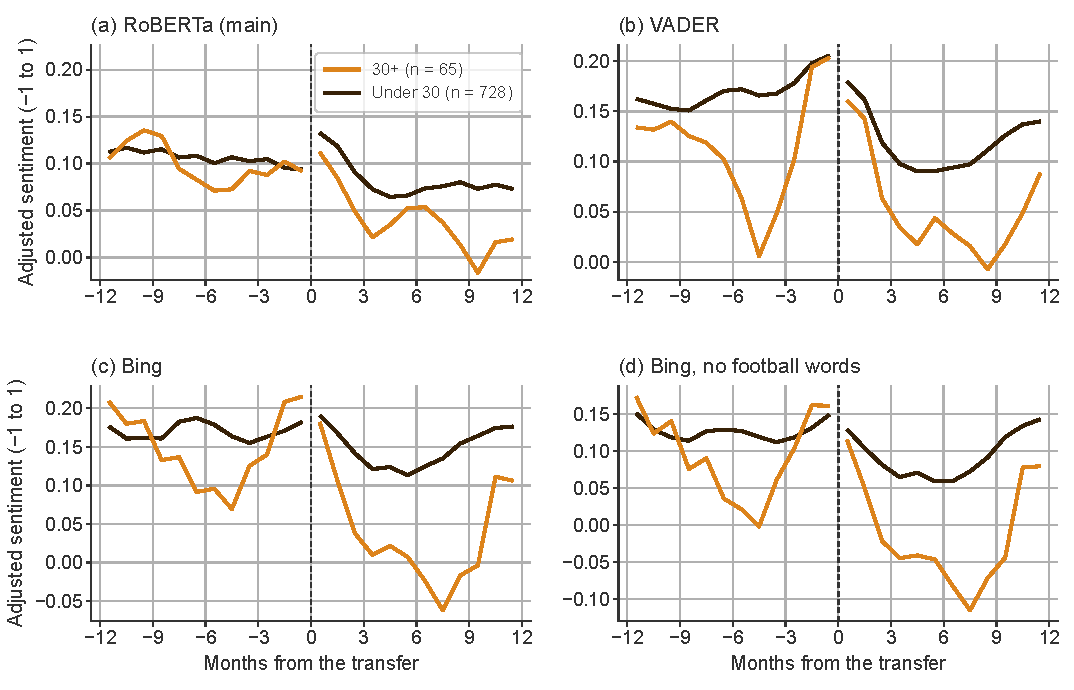
\includegraphics[width=17.8cm]{figures/fig_h2b_arc_paper.pdf}
\caption{Adjusted sentiment of Guardian sentences about Premier League signings, by months from the transfer, for 30+ (orange) and under-30 (blue) signings, under four instruments (A--D). Tone is adjusted as in the all-controls H2b test: quoted sentences dropped, each sentence compared with its article type, and prior coverage, market value and transfer season held at the sample average, so the vertical distance between the lines is the tested gap (printed under each title). Lines: each signing averaged per month, then across signings, 3-month rolling mean; the dashed line is the transfer day ($\pm$7 days excluded). $P$: 5,000 shuffles of the 30+ label within season.}
\label{fig:arc}
\end{figure*}

\subsection*{Older signings receive more coverage}
Coverage volume showed the clearest age difference. Across all 1,332 signings, 30+ signings had 2.2 times as many Guardian articles naming them as under-30 signings in the year before the move (median 27.5 against 12; 95\% interval 1.7--3.0) and 1.4 times as many in the year after (47.5 against 35; 1.1--1.8), with season held fixed (Fig.~\ref{fig:dots}C). At equal market value the ratios were larger, 3.6 and 2.2. Joining the Premier League increased coverage less for older signings: their growth was 0.65 times that of under-30 signings (0.50--0.84; all $P\le0.003$). Even with prior coverage and market value held fixed, 30+ signings received 1.5 times the coverage after the move.

\begin{figure*}[t!]
\centering
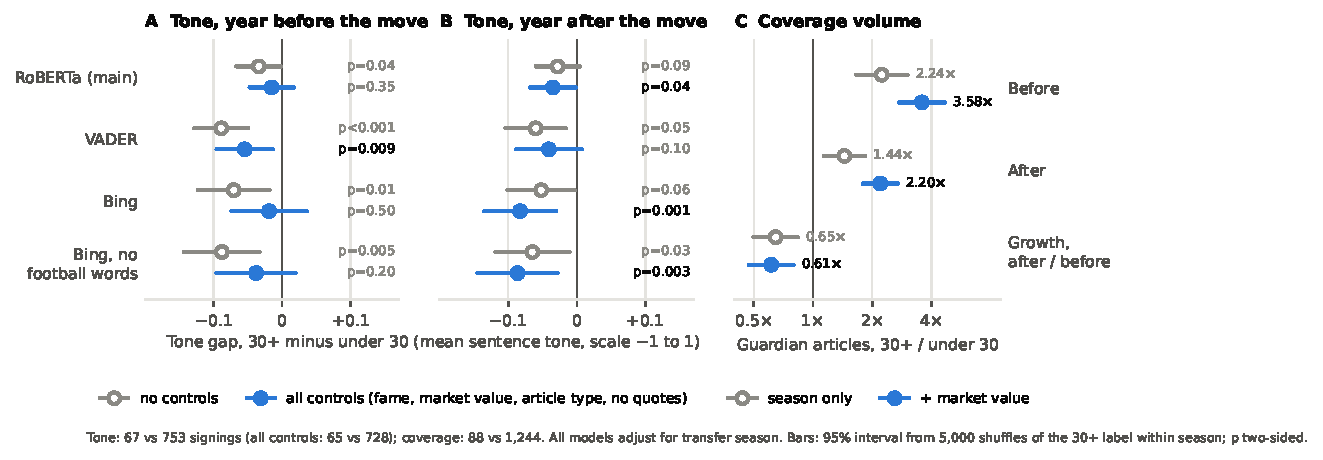
\includegraphics[width=17.8cm]{figures/fig_h2b_tone_coverage.pdf}
\caption{30+ against under-30 signings. (A, B) Tone gap in the year before and after the move under four instruments, without controls (grey, hollow) and with all controls (blue, filled: no quotes, article type, prior coverage, market value, season). (C) Ratio of Guardian articles naming the player, 30+ over under 30, before, after and growth across the move, with season (grey) and also market value (blue) held fixed; log scale. Bars: observed value $\pm1.96$ SD of 5,000 within-season shuffles.}
\label{fig:dots}
\end{figure*}

\section*{Discussion}
\todo{Keep the version of the next paragraph that matches the H1 result, fill in its numbers, delete the other.}

\textcolor{red}{[If 30+ players are less likely to join (H1 supported):]} Older players appear to be at a disadvantage at both stages we measured. Moves that start at a club outside the Premier League end inside it less often when the player is 30 or older \todo{rates, gap, P}, even with origin club and season held fixed, and the older players who do arrive are written about less warmly in their first Premier League year than younger signings of the same fame and price. Access and reception point the same way, although the text data cannot say whether press tone and club decisions influence each other.

\textcolor{red}{[If there is no age gap in joining (H1 not supported):]} Age does not appear to limit access: once origin club and season are held fixed, players aged 30 or older are about as likely as younger players to move into the Premier League \todo{rates, gap, P}. Their reception differs, however: older signings are written about less warmly in their first Premier League year than younger signings of the same fame and price. Whatever disadvantage older players face shows up in how they are covered, not in whether they are signed.

In the Guardian, older Premier League signings are not ignored; they are written about far more than younger players of the same price, before and after they arrive. What differs is how warmly. Before the move, the lower tone around older players is largely what one would expect from players with long, much-reported careers and lower market values. After the move that explanation runs out: at the same prior fame and price, older signings are covered less positively in their first Premier League year. The change across the move itself does not separate the groups, partly because younger signings' tone also falls, and partly because 67 older signings leave the design able to detect only large differences.

These findings carry several limits. Older Premier League signings are few (88; 67 with enough coverage) and bunch in recent seasons (30 in 2022), which we handle by comparing within season but cannot remove. We tried several sets of controls; the after-move gap is consistent in size across them but reaches $P<0.05$ under RoBERTa only once market value is included. The instruments read neutral text as mildly positive and fail on contrasts, and only 14 of the 200 validation sentences concern 30+ players: within those, the instruments did not score older players lower than the labeller did (RoBERTa $+0.14$ for the same human label, $P=0.14$), but the check is weak. Finally, a sentence that names a player is not necessarily about him: 2\% of labelled sentences were about a namesake, and a simple ``main subject'' rule (name in the headline or at least three mentions) was right for only 48\% of articles in a fresh labelled sample, so we do not rely on it for the main results. The analysis covers one newspaper, and the tone it measures is that of the writing, not of readers or fans.

\matmethods{
\subsection*{Transfer network and H1}
\todo{Teammates: data (Transfermarkt transfer file, cleaning: youth/B/reserve clubs, placeholder clubs Without Club/Retired/Career break excluded), network construction (clubs as nodes, directed weighted edges), H1 sample (real club outside the PL that season; outcome = destination in the PL that season; age at transfer, 30+ vs under 30), statistic (difference in joining rates, percentage points), null model (999 shuffles of the age label within origin club and season; one-sided P), robustness.}

\subsection*{Signings and Guardian articles}
Premier League signings were taken from the Transfermarkt data \cite{transfermarkt_kaggle}: a move to a club playing in the Premier League that season, seasons 2012/13--2024/25, market value at least \euro2m, age 18--36 in completed years at the transfer date; same-club moves and loan returns were excluded (paid moves were kept). Age 30+ means 30--36 at the transfer. For each signing we queried the Guardian Content API for the player's full name, accent-free name and known aliases within $\pm$365 days of the transfer, and kept articles that name the player. Name matching handles accents and apostrophes and excludes a name that is part of another person's name (from the 50,149 player names in the Transfermarkt data plus a hand-checked list of coaches and others), and ignores a bare short name when the article also names another person known by it. Sentences were split from the article body; a sentence enters if it names the player, or starts with ``He'' or ``His'' right after one that does.

\subsection*{Sentiment instruments and validation}
VADER gives a compound score in $[-1,1]$; Bing gives (positive $-$ negative words)/(positive $+$ negative words), 0 if none; RoBERTa (\texttt{cardiffnlp/twitter-roberta-base-sentiment-latest}) gives $P(\text{positive})-P(\text{negative})$, inputs truncated at 128 tokens. For validation, 200 sentences (one per article, 100 before and 100 after the move, 151 signings) were sampled from the main sample and labelled without seeing any score, with notes on quotations, contrasts, passing mentions and merged sentences. Six labels marked as unsure were kept; dropping them changes $\rho$ in Table~\ref{tab:validation} by at most 0.02.

\subsection*{Tone per signing and tests}
The main sample excludes liveblogs and match reports and the $\pm$7 days around the transfer. A signing enters if it has at least five scored sentences both before and after. Its tone in a period is the mean of its sentence scores. For H2, the statistic is the difference between the mean change (after minus before) of 30+ and under-30 signings. Its null distribution comes from 5,000 shuffles of the 30+ label among signings within the same transfer season, so that the concentration of older signings in recent seasons cannot stand in for age; $P$ is two-sided, $(1+\#\{|\text{null}|\ge|\text{obs}|\})/5001$ \cite{phipson2010permutation}. Within-group changes were tested by shuffling the period label between whole articles of a signing. For H2b, the same test is applied to the tone in each period. With controls, the statistic is the 30+ coefficient of an ordinary least-squares regression of the signing's tone on season indicators and the controls, refitted for each shuffle; prior coverage is $\log(1+$articles naming the player in the year before$)$ and market value is logged. In the all-controls version, sentences containing quotation marks are dropped and each sentence score is replaced by its difference from the mean of its article type (news, features, comment, \dots) in that period, plus the period mean. Intervals are the observed value $\pm1.96$ SD of the shuffle distribution. Monthly arcs (Fig.~\ref{fig:arc}) average each signing within a month, then across signings, and smooth with a 3-month rolling mean separately before and after the transfer \cite{reagan2016arcs}.

\subsection*{Coverage volume}
For all 1,332 signings, coverage in a period is the number of distinct Guardian articles naming the player. The outcome is $\log(1+$articles$)$, the gap is reported as a ratio, and $P$ comes from the same within-season shuffle with season indicators (and market value and position where stated).
}

\showmatmethods{}

\dataavail{Code for the text part, the selected signings and the hand-labelled samples are in the group repository \todo{link, branch text-pipeline-guardian}. Guardian article text is not redistributed under the Open Platform terms; derived per-signing tone and coverage are provided.}

\acknow{\todo{Acknowledgements, e.g. course staff of DTU 02805.}}
\showacknow{}

\bibsplit[4]
\bibliography{references}

\end{document}
